\documentclass[11pt,notitlepage,a4paper]{article}
%\usepackage[a4paper,hmargin=1.3in,vmargin=1.3in]{geometry}
\usepackage[
  bookmarks=true,       % show bookmarks bar?
  unicode=true,         % non-Latin characters in Acrobat’s bookmarks
  pdftoolbar=false,     % show Acrobat’s toolbar?
  pdfmenubar=false,     % show Acrobat’s menu?
  pdffitwindow=false,   % window fit to page when opened
  pdfstartview={FitH},  % fits the width of the page to the window
  pdftitle={BLAKE3},    % title
  pdfauthor={TODO},     % author
  pdfsubject={BLAKE3},  % subject of the document
  pdfnewwindow=true,    % links in new window
  colorlinks=true,      % false: boxed links; true: colored links
  linkcolor=darkgreen,  % color of internal links
  citecolor=darkblue,   % color of links to bibliography
  filecolor=magenta,    % color of file links
  urlcolor=darkred,     % color of external links
]{hyperref}
\usepackage{url}
%\usepackage{fullpage}
\usepackage{a4wide}
\usepackage{amsmath,amssymb,cite,dsfont}

\usepackage{verbatim,footmisc}
\usepackage{array}
\usepackage{euler}
\usepackage{helvet}
\renewcommand{\familydefault}{\sfdefault}
\fontfamily{phv}\selectfont
\usepackage{multirow}
\usepackage{booktabs}
\usepackage{datetime}
\usepackage{xcolor}
\usepackage{graphicx}
\usepackage{subfigure}

\usepackage[english]{babel}

\usepackage{xspace}
\usepackage{booktabs}
\usepackage{listings}
\usepackage{tikz}
\usepackage[T1]{fontenc} % improves underscore rendering
\usepackage[shortcuts]{extdash} % unbreakable dashes, e.g. SHA\=/2
\usetikzlibrary
{
  calc,
  positioning,
  shapes,
  shapes.geometric,
  arrows
}

\definecolor{darkred}{RGB}{170,0,0}
\definecolor{darkblue}{RGB}{0,0,170}
\definecolor{darkgreen}{RGB}{0,170,0}

\newdateformat{mydate}{\THEYEAR.\twodigit\THEMONTH.\twodigit\THEDAY}

\newcommand{\GG}{\mathsf{G}}
\newcommand{\IV}{\text{IV}}
\newcommand{\cpress}{\text{\textbf{compress}}}
\newcommand{\lto}{\leftarrow}
\newcommand{\BB}{\mathsf{B2}}

\title{BLAKE3}

\begin{document}

\fontfamily{phv}\selectfont

\pagestyle{plain}

%\maketitle
\begin{center}
{\huge BLAKE3: one function, embarrassingly parallel}

\bigskip

\mydate\today 
%%\quad---\quad
% {\large \tt REQUEST FOR COMMENTS, NOT A FINAL VERSION}

\medskip

\url{https://blake3.io}

\medskip

AUTHORS
%Jack O'Connor (\texttt{@oconnor663}) \\
%Jean-Philippe Aumasson (\texttt{@veorq}) \\
%Samuel Neves (\texttt{@sevenps}) \\
%Zooko Wilcox-O'Hearn (\texttt{@zooko}) \\
%Christian Winnerlein (\texttt{@codesinchaos})
\end{center}


\medskip

\begin{center}
  \begin{minipage}{0.92\linewidth}

      \textbf{Abstract.} We present the cryptographic hash function BLAKE3, an
      improved version of BLAKE2 and of its predecessor, the SHA\=/3 finalist
      BLAKE. BLAKE3 supports high degrees of parallelism, using an internal
      tree structure that scales up to any number of SIMD lanes or CPU cores.
      On Intel Kaby Lake, peak single-threaded throughput is 3x that of
      BLAKE2b, 4x that of SHA\=/2, and 8x that of SHA\=/3, and it can scale
      further using multiple threads. At the same time, BLAKE3 is efficient on
      smaller architectures and microcontrollers. Throughput on ARM Cortex-M0
      is 30\% higher than BLAKE2s or SHA\=/256, and 3x that of BLAKE2b,
      SHA\=/512, or SHA\=/3. And unlike BLAKE2 and SHA\=/2, which are divided
      into incompatible variants optimized for different architectures, BLAKE3
      is a single hash function, designed to be consistently fast in software
      across a wide variety of platforms and use cases.

   \end{minipage}
\end{center}

\smallskip

\section{Introduction}\label{sec:intro}

Since its introduction in 2012, BLAKE2 has seen widespread adoption, in large
part because of its strong performance in software. BLAKE2b and BLAKE2s are
included in OpenSSL and in the Python and Go standard libraries. BLAKE2b is
also included as the \texttt{b2sum} utility in GNU Coreutils, and as the
\texttt{generichash} API in Libsodium. And BLAKE2b is the underlying hash
function for Argon2, the winner of the Password Hashing Competition in 2015.

However, a drawback of BLAKE2 has been its large number of incompatible
variants. The original BLAKE2 paper described 64-bit BLAKE2b, 32-bit BLAKE2s,
the parallel variants BLAKE2bp and BLAKE2sp, and a framework for tree modes.
The BLAKE2X paper added extensible output modes. None of these variants are
compatible with each other, and choosing the right one for an application means
understanding both the tradeoffs between them and also the state of language
and library support. BLAKE2b is the most widely supported variant, although it
is rarely the fastest on any particular platform. BLAKE2sp, which has the
highest peak throughput on x86, is sparsely supported and almost never used.

BLAKE3 eliminates this drawback. It is a single hash function with no variants,
designed to support all the use cases of BLAKE2. Furthermore, it improves on
performance, in some cases dramatically. On Intel Kaby Lake, peak throughput on
a single core is triple that of BLAKE2b, and BLAKE3 can scale further to any
number of cores. On ARM Cortex-M0, throughput is 30\% higher than BLAKE2s and
again triple that of BLAKE2b.

Internally, BLAKE3 divides its input into 2 KiB chunks and arranges those
chunks as the leaves of a binary Merkle tree. This tree structure means that
there is no limit to the parallelism that BLAKE3 can exploit, given enough
input. The direct benefit of that parallelism is very high throughput on
systems with SIMD support, including all modern x86 processors. Another benefit
of hashing chunks in parallel is that the implementation can use SIMD vectors
of any width, regardless of the word size of the compression function. That
leaves us free to use a compression function that is efficient on smaller
architectures, without sacrificing performance on x86\=/64.

The BLAKE3 compression function is closely based on BLAKE2s. BLAKE3 has the
same 128-bit security level and 256-bit default output size. The round function
is identical, along with the IV constants and the message schedule. Thus, all
the cryptanalysis of BLAKE2 applies directly to BLAKE3. Based on that analysis
and with the benefit of hindsight, we believe that BLAKE2 is overly
conservative in its number of rounds, and BLAKE3 reduces the number of rounds
from 10 to 7. BLAKE3 also changes the setup and finalization steps of the
compression function to support the internal tree mode, more efficient keying,
and extensible output.

The biggest changes from BLAKE2 and BLAKE3 are:

\begin{itemize}
    \item BLAKE3 has \textbf{no variants or flavors}.
    \item BLAKE3 uses an \textbf{internal tree mode}.
    \item The compression function uses \textbf{fewer rounds}.
    \item In lieu of a parameter block, BLAKE3 provides \textbf{three
        domain-separated public APIs}: \texttt{hash(input)},
        \texttt{keyed\_hash(input, key)}, and \texttt{derive\_key(key,
        context)}.
    \item The space formerly occupied by the parameter block is now used for
        the optional 256-bit key, so \textbf{keying is zero-cost}.
    \item BLAKE3 has direct support for \textbf{extensible output}, which is
        fully parallelizable.
\end{itemize}

\nocite{DBLP:journals/iacr/AumassonNWW13,DBLP:journals/rfc/rfc7693,DBLP:journals/tosc/LuykxMN16}

\section{Specification of BLAKE3}\label{sec:specification}

\subsection{Tree Structure}\label{sec:tree}

BLAKE3 divides the input up into 4096-byte chunks. The final chunk may be shorter, but it's never empty unless the input itself is empty. The chunks are arranged as the leaves of a binary tree. All parent nodes have exactly two children, and the content of each parent node is the hash of its left child concatenated with the hash of its right child. When there's an odd number of nodes in a given level of the tree, the rightmost node is raised to the level above. Here's what the tree looks like as it grows from 1 to 4 chunks.

\begin{figure}[h]
\centering
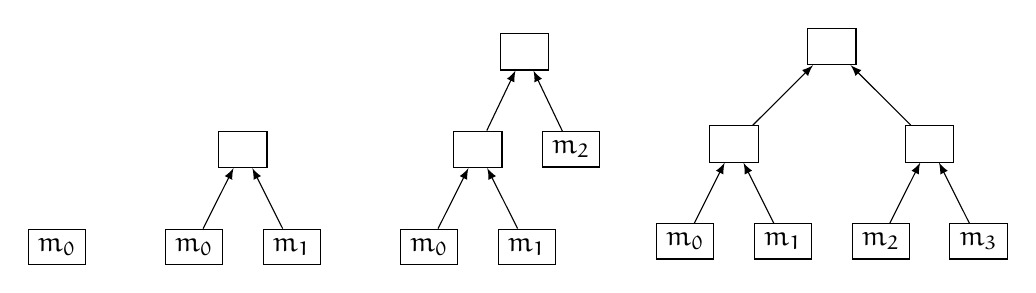
\begin{tikzpicture}

\node[draw,rectangle] (chunk1) at (0, 0) {$m_0$};

%%

\node[draw,rectangle,right=1cm of chunk1] (chunk2) {$m_0$};
\node[draw,rectangle,right=0.5cm of chunk2] (chunk3) {$m_1$};
\node[draw,rectangle,above=1cm of chunk2] (parent1) at ($(chunk2)!0.5!(chunk3)$) {\phantom{$p_0$}};
\draw[-latex] (chunk2) -- (parent1);
\draw[-latex] (chunk3) -- (parent1);

%%

\node[draw,rectangle,right=1cm of chunk3] (chunk2) {$m_0$};
\node[draw,rectangle,right=0.5cm of chunk2] (chunk3) {$m_1$};
\node[draw,rectangle,above=1cm of chunk2] (parent1) at ($(chunk2)!0.5!(chunk3)$) {\phantom{$p_0$}};
\node[draw,rectangle,right=0.5cm of parent1] (chunk4) {$m_2$};
\node[draw,rectangle,above=1cm of chunk4] (parent2) at ($(parent1)!0.5!(chunk4)$) {\phantom{$p_0$}};
\draw[-latex] (chunk2) -- (parent1);
\draw[-latex] (chunk3) -- (parent1);
\draw[-latex] (parent1) -- (parent2);
\draw[-latex] (chunk4) -- (parent2);

%%

\node[draw,rectangle,below right=1cm of chunk4] (chunk2) {$m_0$};
\node[draw,rectangle,right=0.5cm of chunk2] (chunk3) {$m_1$};
\node[draw,rectangle,above=1cm of chunk2] (parent1) at ($(chunk2)!0.5!(chunk3)$) {\phantom{$p_0$}};
\node[draw,rectangle,right=0.5cm of chunk3] (chunk4) {$m_2$};
\node[draw,rectangle,right=0.5cm of chunk4] (chunk5) {$m_3$};
\node[draw,rectangle,above=1cm of chunk4] (parent2) at ($(chunk4)!0.5!(chunk5)$) {\phantom{$p_0$}};
\node[draw,rectangle,above=1cm of parent2] (parent3) at ($(parent1)!0.5!(parent2)$) {\phantom{$p_0$}};
\draw[-latex] (chunk2) -- (parent1);
\draw[-latex] (chunk3) -- (parent1);
\draw[-latex] (chunk4) -- (parent2);
\draw[-latex] (chunk5) -- (parent2);
\draw[-latex] (parent1) -- (parent3);
\draw[-latex] (parent2) -- (parent3);

\end{tikzpicture}
\caption{TODO}\label{fig:fourchunks}
\end{figure}

We can also describe the tree recursively:
\begin{itemize}
\item If a tree/subtree contains 4096 input bytes or less, the tree/subtree is just a chunk.
\item Otherwise, the tree/subtree is rooted at a parent node, and its input bytes are divided between its left and right child subtrees. The number of input bytes on the left is largest power of 2 times 4096 that's strictly less than the total. The remainder, always at least 1 byte, goes on the right.
\end{itemize}

Hashing nodes is done with BLAKE2s, using the following parameters:
\begin{itemize}
\item \textbf{Hash length} is $32$.
\item \textbf{Fanout} is $2$.
\item \textbf{Max} depth is $255$.
\item \textbf{Max} leaf length is $4096$.
\item \textbf{Inner} hash length is $32$.
\item \textbf{Node offset} is incremented for each chunk, i.e., $0$ for the first chunk, $1$ for the second chunk, etc. This counter wraps to zero after reaching the maximum BLAKE2X node offset, $2^{32}-1$. It's $0$ for all parent nodes.
\item \textbf{Node depth} is $0$ for all chunks and $1$ for all parent nodes.
\end{itemize}
In addition, the root node -- whether it's a chunk or a parent -- has the \textbf{last node} finalization flag set to true. Note that BLAKE2 supports setting the last node flag at any time, so hashing the first chunk can begin without knowing whether it's the root.

That root node hash is the output of BLAKE3. Here's an example tree, with 8193 bytes of input that are all zero:
\begin{figure}[h]
\centering
TODO.
\end{figure}

We can verify those values on the command line using the \texttt{blake2} utility from \texttt{blake2\_simd}~\cite{TODO}:
\begin{lstlisting}[basicstyle=\scriptsize\tt,showspaces=false,showstringspaces=false,showtabs=false,breaklines=true,breakatwhitespace=true,language=Bash]
# Install the blake2 utility. Make sure your Cargo bin dir is in your $PATH.
$ cargo install blake2_bin

# Define some aliases for hashing nodes.
$ alias hash_node="blake2 -s --fanout=2 --max-depth=255 --max-leaf-length=4096 --inner-hash-length=32"
$ alias hash_chunk="hash_node --node-depth=0"
$ alias hash_parent="hash_node --node-depth=1"

# Hash the first chunk.
$ first_chunk_hash=`head -c 4096 /dev/zero | hash_chunk --node-offset 0`
$ echo $first_chunk_hash
1f889cb45b1901ce01bba35537ede436e5b84e00327eced603a46a9b2b029506

# Hash the second chunk.
$ second_chunk_hash=`head -c 4096 /dev/zero | hash_chunk --node-offset 1`
$ echo $second_chunk_hash
48d13f5d36b8c94c2d7ce8d59bf7053873f5f2cff8fbccd5c239f4fc752b2f88

# Hash the third chunk.
$ third_chunk_hash=`head -c 1 /dev/zero | hash_chunk --node-offset 2`
$ echo $third_chunk_hash
57e13cda44cdd714424d8ca9c1ae37c3c075ee5c872646eb40c5f58a4ee7cc87

# Define an alias for parsing hex.
$ alias unhex='python3 -c "import sys, binascii; sys.stdout.buffer.write(binascii.unhexlify(sys.argv[1]))"'

# Hash the first two chunks' parent node.
$ left_parent_hash=`unhex $first_chunk_hash$second_chunk_hash | hash_parent`
$ echo $left_parent_hash
7b34f3ebe21be2e02acf0da236f5fa5494653fbf465505e783f43b2dbb826885

# Hash the root node, with the last node flag.
$ unhex $left_parent_hash$third_chunk_hash | hash_parent --last-node
96e2ab1a5486faeaecd306cd7fd7eed78bb48d33de4234b4dd019d481e790c4e

# Verify that this matches the Bao hash of the same input.
$ head -c 8193 /dev/zero | bao hash
96e2ab1a5486faeaecd306cd7fd7eed78bb48d33de4234b4dd019d481e790c4e
\end{lstlisting}

\subsection{Combined Encoding Format}\label{sec:combined}

The combined encoding file format is the contents of the chunks and parent nodes of the tree concatenated together in pre-order (that is a parent, followed by its left subtree, followed by its right subtree), with the 8-byte little-endian unsigned input length prepended to the very front. This makes the order of nodes on disk the same as the order in which a depth-first traversal would encounter them, so a decoder reading the tree from beginning to end doesn't need to do any seeking. Here's the same example tree above, formatted as an encoded file:

\begin{center}
\begin{tabular}{cccccc}
input length & root node & left parent node & first chunk & second chunk & last chunk \\
\texttt{012000...} & \texttt{7b34f3...} & \texttt{1f889c...} & \texttt{000000...} & \texttt{000000...} & \texttt{00}
\end{tabular}
\end{center}

\subsection{Outboard Encoding Format}\label{sec:outboard}

The outboard encoding format is the same as the combined encoding format, except that all the chunks are omitted. In outboard mode, whenever the decoder would read a chunk, it instead reads it from the original input file. This makes the encoding much smaller than the input, with the downside that the decoder needs to read from two streams.

\subsection{Slice Format}

The slice format is very similar to the combined encoding format above. The difference is that the caller requests a specific start point and byte count, and chunks and parent nodes that wouldn't be encountered when seeking to that start point and reading that many bytes are omitted. For example, if we slice the tree above starting at input byte 4096 (the beginning of the second chunk), and request any count of bytes less than or equal to 4096 (up to the end of that chunk), the resulting slice will be this:

TODO

Although slices can be extracted from both combined and outboard encodings, there is no such thing as an ``outboard slice''. Slices always include chunks inline, as the combined encoding does. A slice that includes the entire input is exactly the same as the combined encoding of that input.

Decoding a slice works just like decoding a combined encoding. The only difference is that in cases where the decoder would normally seek forward to skip over a subtree, the slice decoder keeps reading without a seek, since the subtree was already skipped by the slice extractor.

A slice always includes at least one chunk, though in the empty encoding case that chunk is empty. If the requested byte count is zero, that's equivalent to a byte count of one, such that the chunk containing the start point is included in the slice. If the requested start point is at or past the end of the content, the final chunk is included. (See also the ``final chunk requirement'' below.) Apart from that, no parents or chunks after the end of the requested bytes are included. Either the slice extractor or the slice decoder may return an error if the requested bytes exceed the end of the content (strict bounds checking), or they may cap the requested bytes (permissive bounds checking). The reference implementation is permissive.

\subsection{Decoder}

After parsing the length from the first eight bytes of an encoding, the decoder traverses the tree by reading parent nodes and chunk nodes. The decoder verifies the hash of each node as it's read, and it may return the contents of each valid chunk to the caller immediately. The length itself is considered validated when and only when the decoder validates the final chunk, either by validating the entire encoding or by seeking to the end and validating only the right edge of the tree. The decoder must not expose the length to the caller in any way before the final chunk is validated. There are a number of ways the decoder might expose the length, some of which are less obvious than others:
\begin{itemize}
\item An explicit \texttt{.length()} method. The reference implementation doesn't include one, because it would be required to seek internally. Callers who need the length in advance will usually do better to store it separately along with the hash.
\item Reading the empty encoding. Any read of the empty encoding reports EOF, thereby exposing the length (zero). The decoder must verify that the final chunk (that is, the empty chunk) matches the root hash. Most implementations will naturally satisfy this requirement for non-empty encodings as part of reading chunk bytes, but it's easy to forget it in the empty case by assuming that you're finished whenever the current position equals the content length.
\item Seeking past the end. If I seek to an offset greater than or equal to the content length, the next read will return EOF, exposing the length. That means either the seek itself or the following read must have validated the final chunk.
\item Seeking relative to the end. Most seek implementations support something akin to \texttt{SeekFrom::End}. That exposes the length through the absolute offset returned by the seek, which means the seek itself must validate the final chunk.
\end{itemize}
For decoders that don't expose a \texttt{.length()} method and don't support seeking, the security requirements can be simplified to ``verify the hash of every node you read, and don't skip the empty chunk.'' But decoders that do support seeking need to consider the final chunk requirement very carefully. The decoder is expected to maintain these guarantees, even in the face of a man-in-the-middle attacker who modifies the encoded bytes:
\begin{itemize}
\item Any output byte returned by the decoder matches the corresponding input byte from the original input.
\item If EOF is indicated to the caller in any way, either through a read or through a seek, it matches the length of the original input.
\item If the decoder reads a complete output to EOF, the decoding hash must be the BLAKE3 hash of that output. There are no ``decoding collisions'' where two different hashes decode the same output to EOF. (Though two different hashes may decode the same output, if at least one of the decodings encounters an error before EOF.)
\end{itemize}
Note one non-guarantee in particular: The encoding itself may be malleable. Multiple ``different'' encodings may decode to the same input, under the same hash. See the design rationales for more on this.

\section{Security}\label{sec:security}

When designing a tree mode, there are pitfalls that can compromise the security of the underlying hash. For example, if one input produces a tree with bytes X at the root node, and we choose another input to be those same bytes X, do those two inputs result in the same root hash? If so, that's a hash collision, regardless of the security of the underlying hash function. Or if one input results in a root hash Y, could Y be incorporated as a subtree hash in another tree without knowing the input that produced it? If so, that's a length extension, again regardless of the properties of the underlying hash. There are many possible variants of these problems.

Daemen et al.~\cite{DBLP:journals/ijisec/BertoniDPA14,DBLP:journals/tosc/DaemenMA18} lays out a minimal set of requirements for a tree mode, to prevent attacks like the above. This section describes how BLAKE3 satisfies those requirements. They are:
\begin{enumerate}
\item \textbf{Tree decodability.} The exact definition of this property is fairly technical, but the gist of it is that it needs to be impossible to take a valid tree, add more child nodes to it somewhere, and wind up with another valid tree. That is, it shouldn't be possible to interpret a leaf node as a parent node, or to add more children to an existing parent node.
\item \textbf{Message completeness.} It needs to be possible to reconstruct the original message unambiguously from the tree.
\item \textbf{Final-node separability.} Again the exact definition is fairly technical, but the gist is that it needs to be impossible for any root node and any non-root node to have the same hash.
\end{enumerate}
We ensure \textbf{tree decodability} by domain-separating parent nodes from leaf nodes (chunks) with the \textbf{node depth} parameter. BLAKE2's parameters are functionally similar to the frame bits used in the paper, in that two inputs with different parameters always produce a different hash, though the parameters are implemented as tweaks to the IV rather than by concatenating them with the input. Because chunks are domain-separated from parent nodes, adding children to a chunk is always invalid. That, coupled with the fact that parent nodes are always full and never have room for more children, means that adding nodes to a valid tree is always invalid.

\textbf{Message completeness} is of course a basic design requirement of the encoding format. Concatenating the chunks in order gives the original message.

We ensure \textbf{final-node separability} by domain-separating the root node from the rest of the tree with the \textbf{last node} flag. BLAKE2's last node flag is similar to its other parameters, except that it's an input to the last call to the compression function rather than a tweak to the IV. In practice, that allows an implementation to start hashing the first chunk immediately rather than buffering it, and to set the last node flag at the end if the first chunk turns out to be the only chunk and therefore the root.

That framework concerns the security of the hash function. To reason about the security of the decoder, we can start by observing that decoding verifies the hash of almost every part of the encoded file. If the hash function is collision resistant, then these parts of the encoding can't be mutated without leading to a hash mismatch. The one part that isn't directly verified is the length header. The possibility that the length header might be mutated leads to the final chunk requirement above. If the length is increased, that's guaranteed to either lengthen the final chunk, or to replace the final chunk with another parent node. Likewise if the length is decreased, that's guaranteed to either shorten the final chunk, or to replace one of the parent nodes along the right edge of the tree with a chunk. All four of those scenarios are guaranteed to cause a hash mismatch, because of the collision resistance of BLAKE2s and because of the domain separation between parents and chunks, as long as the decoder validates the final chunk. The design rationales discuss further why we prefer to rely on this final chunk requirement rather than hashing the length as associated data.

\section{Storage Requirements}\label{sec:storage}

A BLAKE3 implementation needs to store one hash ($32$ bytes) for every level of the tree. The largest supported input is $2^{64} - 1$ bytes. Given the $4096$-byte chunk size ($2^{12}$), that's $2^{52}$ leaf nodes, or a maximum tree height of $52$. Storing $52$ hashes, $32$ bytes each, requires $1664$ bytes, in addition to the $168$ bytes required by BLAKE2s. For comparison, the TLS record buffer is $16384$ bytes.

Extremely space-constrained implementations that want to use BLAKE3 have to define a more aggressive limit for their maximum input size. In some cases, such a limit is already provided by the protocol they're implementing. For example, the largest possible IPv6 ``jumbogram'' is $4$\,GiB. Limited to that maximum input size, BLAKE3's storage overhead would be $20$ hashes or $640$ bytes.


\section{Performance}\label{sec:performance}

To get the highest possible throughput, the reference implementation uses both multithreading and SIMD instructions. Threading exploits the multiple cores available on modern CPUs, and SIMD allows each thread to hash multiple chunks in parallel for much higher throughput per thread.

Multithreading in the current implementation is done with the join function from the Rayon library. It splits up its input recursively -- an excellent fit for traversing a tree -- and allows worker threads to ``steal'' the right half of the split, if they happen to be free. Once the global thread pool is initialized, this approach doesn't require any heap allocations.

There are two different approaches to using SIMD to speed up BLAKE2. The more common way is to optimize a single instance, and that's the approach that just beats SHA-1 in the BLAKE2b benchmarks. But the more efficient way, when you have multiple inputs, is to run multiple instances in parallel on a single thread. Samuel Neves discussed the second approach in a 2012 paper and implemented it in the reference AVX2 implementation of BLAKE2sp. The overall throughput is more than triple that of a single optimized BLAKE2s instance. The \texttt{blake2s\_simd} implementation includes a \texttt{hash\_many} interface, which provides the same speedup for multiple instances of BLAKE2s, and BLAKE3 uses that interface to make each worker thread hash multiple chunks in parallel. Note that the main downside of BLAKE2sp is that it hardcodes 8-way parallelism, such that moving to a higher degree of parallelism would change the output. But \texttt{hash\_many} doesn't have that limitation, and when AVX-512 becomes more widespread, it will execute 16-way parallelism without changing the output or the API.

\section{Rationale}\label{sec:rationale}

TODO

\bibliographystyle{plainurl}
\bibliography{blake3}

\end{document}
